\documentclass[10pt,a4paper]{beamer}
\usepackage[utf8]{inputenc}
\usetheme{Boadilla}
\usepackage{amsmath}
\usepackage{amsfonts}
\usepackage{graphicx}
\usepackage{tikz}
\usetikzlibrary{snakes}
\usepackage{amssymb}
\usepackage{enumitem}
\title{Semaine 12 : Marché des titres adossés à des créances \\ $(2^{e}$ partie)}
\date{2021-04-07} 
\author{Simon-Pierre}
\institute{Université Laval}

\begin{document}
\begin{frame}
\titlepage
\end{frame}

\begin{frame}
\tableofcontents
\end{frame}

\section{Hypothèque résidentiel}

\begin{frame}{Le marché hypothécaire résidentiel}
Le marché des prêts hypothécaires résidentiels peut être divisé en deux sous-secteurs en fonction de la qualité de crédit de l'emprunteur:
\begin{enumerate}[label=\arabic*)]
\item Prime mortgage market 
\begin{itemize}[label=\bullet]
\item Les prêts qui satisfont aux normes de souscription
\item Les prêts qui ne sont pas conformes pour une raison autre que la qualité du crédit ou parce que le prêt n'est pas de premiers rang
\end{itemize}
\item Subprime mortgage market. 
\begin{itemize}[label=\bullet]
\item Les prêts accordés aux emprunteurs dont la cote de crédit est dégradée ou lorsque le prêt est de second rang
\end{itemize}
\end{enumerate}
\end{frame}

\section{La Titrisation}

\begin{frame}{La Titrisation}
\begin{block}{Intermediation du crédit (Ancien système)}
\begin{itemize}[label=\bullet]
\item La banque commercial emprunte et prête de l’argent
\item Le risque de défaut est dans les mains de la banque
\item La banque doit charger pour:
\begin{itemize}[label=\bullet]
\item Pertes possibles
\item Manque de liquidité $\rightarrow$ impossible d'éliminer le risque
\end{itemize}
\end{itemize}
\end{block}
\end{frame}


\begin{frame}{La Titrisation}
\begin{block}{Désintermediation du crédit (Nouveau système)}
\begin{itemize}[label=\bullet]
\item Les investisseurs (ou agences fédérales) partagent une partie du risque de crédit
\item Chaque investisseur détient une petite partie du risque
\item L’actif est liquide
\item Le prêt peut être \textbf{packaged} en différent tranches pour satisfaire différent type d’investisseurs.
\item Résultat $\rightarrow$ financement moins cher
\end{itemize}
\end{block}
\end{frame}

\begin{frame}{Pool de prêt hypothécaire}
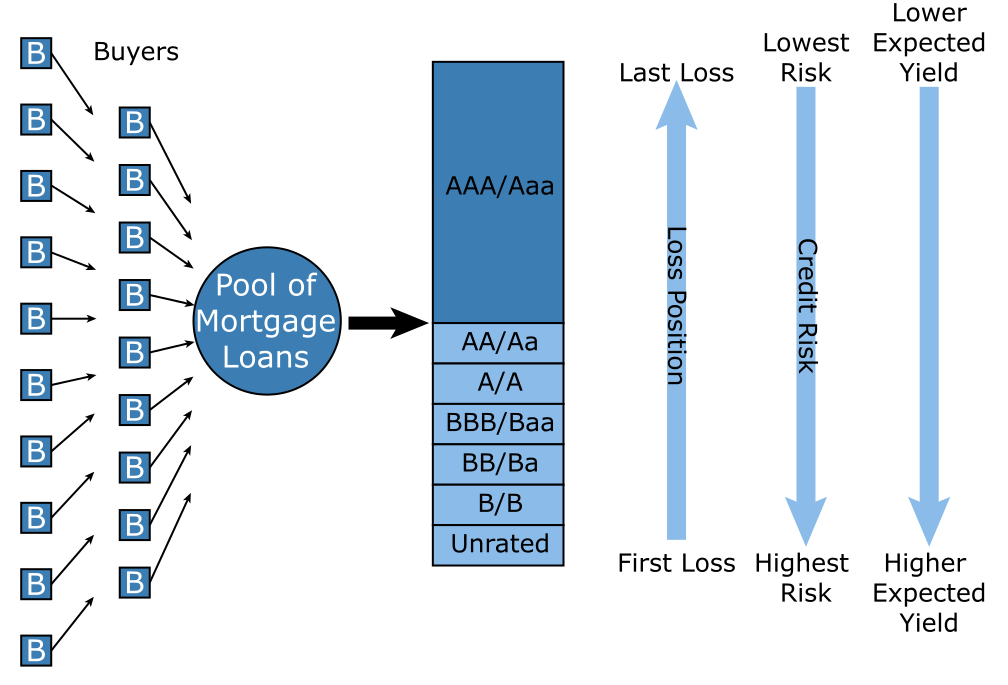
\includegraphics[width=110mm]{Pool}
\end{frame}

\section{Mortgage Passthrough Securities}

\begin{frame}{Mortage Backed Securities (MBS)}
\begin{itemize}[label=\bullet]
\item Hypothèque : titre peu liquide car non standardisé (titre OTC entre le préteur et l’emprunteur)
\item MBS : titre de dette garanti par un panier de prêt résidentiels. 
\item Les MBS transforme les hypothèques en titres liquides.
\item Les \textbf{agency securities} sont des MBS émis par les agences gouvernementales:
\begin{itemize}[label=\bullet]
\item Fannie Mae
\item Freddie Mac
\end{itemize}
\end{itemize}
\end{frame}

\begin{frame}{Mortgage Passthrough Securities}
\begin{itemize}[label=\bullet]
\item Un MPS représente une part d’un pool d’hypothèques
\item Les hypothèques inclus dans le pool sont titrisées.
\item Les investisseurs du pool hypothécaire reçoivent des paiements mensuels issus par le pool.
\item Ces paiements sont moindres que les mensualités reçues par le pool (frais de service, garantie, assurance)
\item Les MPS sont transigées sur le marchés secondaire: les hypothèques sont ainsi converties en titres liquides
\item Le timing des paiements hypothécaires reçus par le pool ne coïncide pas avec les versements : 
\begin{itemize}[label=\bullet]
\item il y a un délai pour le transfert de l’argent.
\end{itemize}
\end{itemize}

\end{frame}

\begin{frame}{Mortgage Passthrough Securities}
\begin{block}{Les conventions de prépaiements et les flux monétaires}
\begin{itemize}[label=\bullet]
\item Les prépaiements rends les flux monétaires des MBS incertains.
\item Pour évaluer un MPS, il faut poser des conditions quant aux condition de prépaiement les hypothèques du pool.
\item Deux normes de l’industrie:
\begin{itemize}[label=\bullet]
\item Le taux de prépaiement conditionnel
\item Le benchmark de prépaiement de la \textbf{Public Securities Association}
\end{itemize}
\end{itemize}
\end{block}
\end{frame}


\begin{frame}{Mortgage Passthrough Securities}
\begin{block}{Taux de prépaiement conditionnel}
\begin{itemize}[label=\bullet]
\item Le taux de prépaiement conditionnel (\textbf{conditional Prepayment Rate, CPR})
\item C’est le taux annuel auquel la valeur résiduelle d’un pool d’hypothèque est prépayée durant la vie du pool
\item Le CPR peut-être converti en taux de mortalité mensuel ( \textbf{Single-Monthly Mortality Rate, SMM})
\begin{align*}
SMM=1-(1-CPR)^{1/12}
\end{align*}
\item On peut ainsi calculer la valeur des prépaiements attendue
\begin{align*}
P_m=SMM \times (RV-M)
\end{align*}
\end{itemize}
Où $P_m$ est un prépaiements au temps $m$,  $RV$ est la valeur résiduelle au début du mois et $M$ est le montant des mensualités régulières pour le mois.
\end{block}
\end{frame}


\begin{frame}{Mortgage Passthrough Securities}
\begin{block}{Public Securities Association (PSA)}
\begin{itemize}[label=\bullet]
\item Le benchmark de prépaiement de la \textbf{Public Securities Association (PSA)}.
\item Le PSA assume que le montant de prépaiement pour un pool d’hypothèque augmente au fur et à mesure que le pool vieillit, ou qu’il devient saisonnier.
\item Le benchmark est 100 PSA
\item Un pool hypothécaire peut présenter des taux de prépaiement plus rapides ou plus lents que 100\% PSA (cela dépend du taux de coupon et du niveau des taux d’intérêt).
\end{itemize}
\end{block}
\begin{block}{Interprétation}
\begin{itemize}[label=\bullet]
\item 50\%PSA = 50\% CPR prescrit par 100\% PSA
\item 150\% PSA = 150\% CPR prescrit par 100\%PSA
\end{itemize}
\end{block}
\end{frame}


\begin{frame}{Mortgage Passthrough Securities}
\begin{block}{Les facteurs influençant le prépaiement}
\begin{itemize}[label=\bullet]
\item Le taux hypothécaire
\item Les caractéristiques du prêt hypothécaire
\item Le risque d’extension et le risque de contraction
\item La durée de vie moyenne
\end{itemize}
\end{block}
\end{frame}


\begin{frame}{Mortgage Passthrough Securities}
\begin{block}{La durée de vie moyenne}
\begin{itemize}[label=\bullet]
\item En tenant compte du risque de prépaiement, la maturité réelle des MPS n’est pas égale à la maturité du contrat
\item Les investisseurs calculent la durée de vie moyenne (\textbf{Average Life ou Weighted Average Life}).
\end{itemize}
\begin{align*}
\textbf{Average Life}=\sum_{t=1}^T \frac{t \times(\textbf{Principal attendu à la date t})}{12 \times(\textbf{Principal total})}
\end{align*}
\begin{itemize}[label=\bullet]
\item Quand les taux hypothécaire baissent, la durée de vie moyenne diminue (\textbf{risque de contraction})
\item Quand les taux montent, la durée de vie moyenne augmente (\textbf{risque d’extension})
\end{itemize}
\end{block}
\end{frame}


\begin{frame}{Mortgage Passthrough Securities}
\begin{block}{Les obligations hypothécaires garanties}
\begin{itemize}[label=\bullet]
\item Les obligations hypothécaires garanties (\textbf{Collateralized Mortgage Obligations, CMO})
\item Les CMO sont des parts d’un pool hypothécaire dont les flux monétaires sont alloués selon différentes classes, ou tranches, chacune ayant un droit de regard différents sur les actifs du pool.
\item Ainsi les investisseurs peuvent choisir des CMO selon leur classe, dépendamment du degré d’exposition voulu au risque de contraction et d’extension.
\end{itemize}
\end{block}
\end{frame}

\begin{frame}{Mortgage Passthrough Securities}
\begin{block}{Les trois types de CMO les plus connus}
\begin{itemize}[label=\bullet]
\item interest-only (\textbf{IOs}) and principal-only (\textbf{POs}) strips

\item sequential CMOs

\item protected amortization class securities (\textbf{PACs})
\end{itemize}
\end{block}
\end{frame}


\begin{frame}{Mortgage Passthrough Securities}
\begin{block}{Les trois types de CMO les plus connus}
\begin{itemize}[label=\bullet]
\item interest-only (\textbf{IOs}) and principal-only (\textbf{POs}) strips
\item sequential CMOs
\item protected amortization class securities (\textbf{PACs})
\end{itemize}
\end{block}
\end{frame}

\section{Sequential CMOs}

\begin{frame}{Sequential CMOs}
\begin{itemize}[label=\bullet]
\item Les CMO séquentiels découpent un pool de prêts hypothécaires en un certain nombre de tranches.

\vspace{0.5cm}

\item Chaque tranche donne droit à une part du capital du pool hypothécaire et des intérêts sur cette part du principal.

\vspace{0.5cm}

\item Les flux de trésorerie sont distribués séquentiellement, de manière à créer des titres avec une gamme d'échéances.
\end{itemize}
\end{frame}

\begin{frame}{Sequential CMOs}
\begin{block}{Les flux de trésorerie sont transmis comme suit:}
\begin{itemize}[label=\bullet]
\item Tous les paiements de principal iront à la tranche la plus élevée (\textbf{par ordre alphabétique}), jusqu'à ce que tout le principal de cette tranche ait été remboursé.
\item Toutes les tranches reçoivent des paiements d'intérêts proportionnels.
\end{itemize}
\end{block}

\begin{block}{Tranche Z}
Les intérêts sur le principal de la tranche Z sont payés en espèces à la tranche la plus élevée en échange d'un transfert d'un montant égal de principal, jusqu'à ce que tout le principal de la tranche la plus élevée ait été entièrement remboursé.
\end{block}
\end{frame}

\section{Protected amortization class (PAC) bonds}

\begin{frame}{Protected amortization class (PAC) bonds}
\begin{itemize}[label=\bullet]
\item Les obligations de la classe d'amortissement protégé (PAC) sont prioritaires pour les paiements périodiques du principal.

\vspace{0.5cm}


\item Les flux de trésorerie résiduels sont versés à des obligations de soutien PAC (ou compagnons).

\vspace{0.5cm}

\item Les flux de trésorerie PAC sont prévisibles tant que les paiements anticipés restent dans une fourchette spécifiée.
\end{itemize}
\end{frame}


\section{Stripped MBS}

\begin{frame}{Stripped MBS}
\begin{block}{Principal-Only Strip (PO):}
\begin{itemize}[label=\bullet]
\item Vendu à escompte par rapport à la valeur nominale
\vspace{0.3cm}
\item Les flux monétaires sont bas au début et augmentent au fur et à mesure que la composante remboursement de capital prend de l’ampleur dans les paiments hypothécaires.
\vspace{0.3cm}
\item La performance d’un PO est extrêmement sensible aux taux de prépaiement.
\vspace{0.3cm}
\item Le prix des PO augmentent dans un environnement de baisse des taux d’intérêt
\end{itemize}
\end{block}

\end{frame}


\begin{frame}{Stripped MBS}
\begin{block}{Interest-Only Strips (IO):}
\begin{itemize}[label=\bullet]
\item Les flux monétaires sont haut au début et déclinent au fur et à mesure que la composante remboursement de capital prend de l’ampleur par rapport au paiments hypothécaires total
\vspace{0.3cm}
\item Les investisseurs veulent des taux de prépaiements bas : l’intérêt est calculé sur la valeur résiduelle de l’hypothèque au début de la période de paiement.
\vspace{0.3cm}
\item Le prix des IO suit le mouvement des taux d’intérêt
\end{itemize}
\end{block}

\end{frame}

\end{document}